% Provenance (never printed): see sources/outline_sources.md (Year 2: taphonomy; index fossils;
% facies and fossils as environment markers; reconstructing a palaeoenvironment from a map and a
% section). Taphonomy after Loron (2024); live, dead and fossil assemblages after Tyler and
% Kowalewski (2025); Lagerstaetten after Gaines and others (2024), Mussini and Butterfield
% (2025), Vannier and others (2018), Gerschermann and others (2021) and Rauhut and others
% (2018); zone durations after Al-Suwaidi and others (2022); ichnofacies after Buatois and others
% (2020) and Paz and others (2023); stenohaline groups after McGairy and others (2021) and Saleh
% and others (2022). The Varden column from figdata/shared/region.py; porosities and rates from
% figdata/bachelor-2/palaeoenv.py; exercise and problem values in the Book 4 scratch calculator
% calc/ch20.py. The fossil content given to the Varden units is invented, like the region.
\chapter{Fossils and Palaeoenvironments}\label{ch:b2:palaeoenvironments}

On a slab of grey sandstone lie three clues: the trail a trilobite ploughed through the mud,
the ripples a current left behind, and a burrow that a worm dug and abandoned. None of them is a
whole animal, and yet together they say that this hillside was once the floor of a sea, shallow
enough for waves to stir it, salty enough for trilobites to live in it. Fossils are the
remains and the traces of past life, and geologists read them twice: as clocks that date the rock,
and as witnesses of the place where it formed. This chapter follows a living thing from its death
to the collector's drawer, opens the rare deposits where even soft bodies survive, and then reads
the environment of a vanished sea, with numbers, in the cover of the Varden Hills.
% ledger: usgs:fossil-record-bulk, loron24:taphonomy

\begin{recall}
\textbf{From the school volumes}: fossil, mould, cast and \omterm{def:b2:palaeoenvironments:fossil-kinds}{trace fossil}; how burial and minerals
turn a shell to stone; the succession of fossils through time. \textbf{From the Year 1 volume}:
sedimentary facies and depositional environments, turbidites, reefs and ooids; biozones, index
fossils and first appearance datums; compaction, decompaction, Athy's law and the solid thickness
of a layer; cement; accommodation. \textbf{From earlier chapters}: transgressions and regressions,
the long-term sea level and the \omterm{def:b2:phanerozoic-earth:oae}{oceanic anoxic events} (\cref{ch:b2:phanerozoic-earth}). How
species evolve, and how animals and plants are classified, belong to the biology books.
\end{recall}

\section{From death to fossil}\label{sec:b2:palaeoenvironments:taphonomy}

Most living things leave nothing behind. Bacteria and scavengers consume the soft parts within
days or years, currents break and scatter the hard ones, and the acids of soils and pore waters
dissolve what is left. A fossil is what survives all of these, and survives again the burial,
the heating and the uplift of the rock that holds it.

\begin{definition}[Taphonomy; preservation potential]\label{def:b2:palaeoenvironments:taphonomy}
\emph{Taphonomy}\index{taphonomy} is the study of what happens to the remains of an organism
from its death to its discovery as a fossil: decay, scavenging, transport, burial, and the
chemical changes of diagenesis. The \emph{preservation potential}\index{preservation potential}
of an organism, or of one of its parts, is the probability that it passes through these stages
and survives in the rock.
\end{definition}
% ledger: loron24:taphonomy

Every stage removes something, adds something, or changes something. Decay and scavenging remove
soft tissues; minerals from the pore water fill the pores of a bone or replace the aragonite of a
shell, adding matter that the animal never had; heating alters the organic molecules that remain.
Loron sorts all these post-mortem changes into three kinds, gain, loss and alteration, and
writes them as one equation for the change of any measurable feature between an organism and its
fossil. The figure below follows the stages and what each takes away.
% ledger: loron24:taphonomy

\begin{omfigure}
\centering
\begin{tikzpicture}[font=\scriptsize, x=1cm, y=1cm,
  stage/.style={draw=black!60, fill=omSea!12, rounded corners=2pt, align=center,
    text width=2.05cm, minimum height=1.25cm, inner sep=2pt},
  loss/.style={align=center, text width=2.05cm, text=omThm!80!black}]
\node[stage] (a) at (0,0) {\textbf{death}\\a living\\community};
\node[stage] (b) at (2.75,0) {\textbf{decay and}\\\textbf{scavenging}\\on the floor};
\node[stage] (c) at (5.5,0) {\textbf{transport}\\currents sort\\and break};
\node[stage] (d) at (8.25,0) {\textbf{burial}\\below the\\active layer};
\node[stage] (e) at (11,0) {\textbf{diagenesis}\\compaction,\\replacement};
\node[stage] (f) at (13.75,0) {\textbf{exhumation}\\and\\collection};
\foreach \u/\v in {a/b, b/c, c/d, d/e, e/f} {\draw[-{Stealth[length=2mm]}, black!70] (\u) -- (\v);}
\node[loss, anchor=north] at (2.75,-0.8) {soft tissue lost;\\skeletons fall apart};
\node[loss, anchor=north] at (5.5,-0.8) {light parts carried off,\\shells broken};
\node[loss, anchor=north] at (8.25,-0.8) {slow burial: more\\time for the losses};
\node[loss, anchor=north] at (11,-0.8) {aragonite dissolved,\\minerals added};
\node[loss, anchor=north] at (13.75,-0.8) {eroded away,\\or never found};
\end{tikzpicture}
\par\smallskip{\small The taphonomic path from a living community to a collection, with what
each stage removes or changes. Burial is the turning point: before it the remains are exposed to
every loss; after it, only diagenesis and erosion act on them.}
\end{omfigure}
% ledger: loron24:taphonomy

The school volumes called a fossil any remains or trace of past life kept in rock. The two kinds
behave so differently in the rock that they deserve their own names.

\begin{definition}[Body fossil; trace fossil]\label{def:b2:palaeoenvironments:fossil-kinds}
A \emph{body fossil}\index{body fossil} is part of the body of an organism, or the mould or cast
of that part: a shell, a bone, a tooth, a leaf, and in rare deposits a soft tissue. A
\emph{trace fossil}\index{trace fossil} is a structure that an organism made by its activity in or
on a sediment or a rock: a track, a trail, a burrow, a boring, a feeding pattern.
\end{definition}

A \omterm{def:b2:palaeoenvironments:fossil-kinds}{trace fossil} is part of the sediment it was dug in: a current that moved it would destroy it.
It therefore records the conditions of the very place where its maker lived, which a shell,
easily rolled along the floor, does not always do. \omterm{def:b2:palaeoenvironments:fossil-kinds}{Trace fossils} are named like organisms, with a
genus and a species, but the name describes the structure, not the animal: the same burrow can be
dug by several kinds of animal, and one animal can leave several kinds of trace.

\subsection*{Burial against destruction}

The race between burial and destruction can be put into a simple model. Remains lying on the
floor are destroyed at a constant rate $k$, the probability per unit time that they are eaten,
broken up or dissolved; they are safe once a thickness $h$ of sediment covers them; and the
sediment accumulates at the rate $s$.

\begin{proposition}[Burial before destruction]\label{prop:b2:palaeoenvironments:burial}
Under these assumptions, the probability that a remain reaches safety is
\[
  P = e^{-kh/s}.
\]
It depends on the three quantities only through the ratio of the time to burial, $h/s$, to the
mean survival time on the floor, $1/k$.
\end{proposition}

\begin{proof}
The remain needs the time $T = h/s$ to be covered by the thickness $h$. With a constant rate of
destruction $k$, the probability $p(t)$ of surviving to the time $t$ obeys $p' = -kp$, $p(0) =
1$, so that $p(t) = e^{-kt}$; at $t = T$ this is $e^{-kh/s}$.
\end{proof}

\begin{example}[A shell on a quiet floor]\label{ex:b2:palaeoenvironments:shell}
Suppose a shell survives on the floor for 20 years on average, $k = \qty{0.05}{yr^{-1}}$, and is
safe under $h = \qty{0.1}{m}$ of mud. At $s = \qty{1}{mm.yr^{-1}}$ the time to burial is 100
years and $P = e^{-5} = 0.0067$: fewer than one shell in a hundred survives. At
\qty{1}{cm.yr^{-1}}, $P = e^{-0.5} = 0.61$. A storm that dumps \qty{0.3}{m} of sand in a day
buries everything at once, and then $P$ is close to one. The numbers are assumed, but the lesson
is not: fossils gather where sediment arrives fast or in sudden beds.
\end{example}

The model also shows why the record is biased. A soft-bodied worm, whose mean survival time on
the floor is days rather than decades, has a value of $k$ hundreds of times larger than a thick
shell, and so an exponentially smaller chance. The bulk of the fossil record is made of animals
with shells and of microscopic remains. Tyler and Kowalewski tested how much a community loses on
its way into the rock. At 51 sites of a coastal sea floor they counted 135 living species of
invertebrates, 150 species among the shells and skeletons lying dead on the floor, and 112 that
also have a fossil record. The dead outnumber the living because the shells on the floor gathered
over many years, from animals that no longer live there. Detritivores and carnivores, mostly
soft-bodied, are the least likely to be preserved; yet the main ecological groups of the living
community were all found again among the dead.
% ledger: usgs:fossil-record-bulk, tyler25:live-dead, tyler25:soft-bodied

\section{Windows of exceptional preservation}\label{sec:b2:palaeoenvironments:lagerstatten}

\begin{definition}[Lagerstätte]\label{def:b2:palaeoenvironments:lagerstatte}
A \emph{Lagerstätte}\index{Lagerstätte} (plural Lagerstätten) is a sedimentary deposit that
preserves fossils of exceptional quality, in particular the soft, non-biomineralised tissues that
decay destroys almost everywhere else; such a deposit is also called a Konservat-Lagerstätte.
\end{definition}
% ledger: gaines24:konservat

Lagerstätten are rare, but much of what is known of soft-bodied animals comes from them, and
the first great radiation of animals, in the Cambrian, is best understood from them.
% ledger: gaines24:konservat

\subsection*{The Burgess Shale}

In 1909 Charles Walcott sketched in his field book a small arthropod he had found in the Burgess
Shale of British Columbia. He later collected hundreds of
specimens of it, \emph{Waptia}, from a single interval about \qty{2}{m} thick, the Phyllopod
Bed; its modern description rests on more than 1800 specimens kept in two museums. The Burgess
Shale, about 508 million years old, was laid down in deeper water, facing a steep submarine
escarpment. Its fossils include animals without shells, preserved as flattened films of carbon,
often whole bodies. Such preservation is tied to burial in oxygen-poor muds that animals did not
burrow and currents did not rework: the losses of the figure above were stopped at once.
% ledger: vannier18:waptia, mussini25:burgess

\begin{omfigure}
\centering
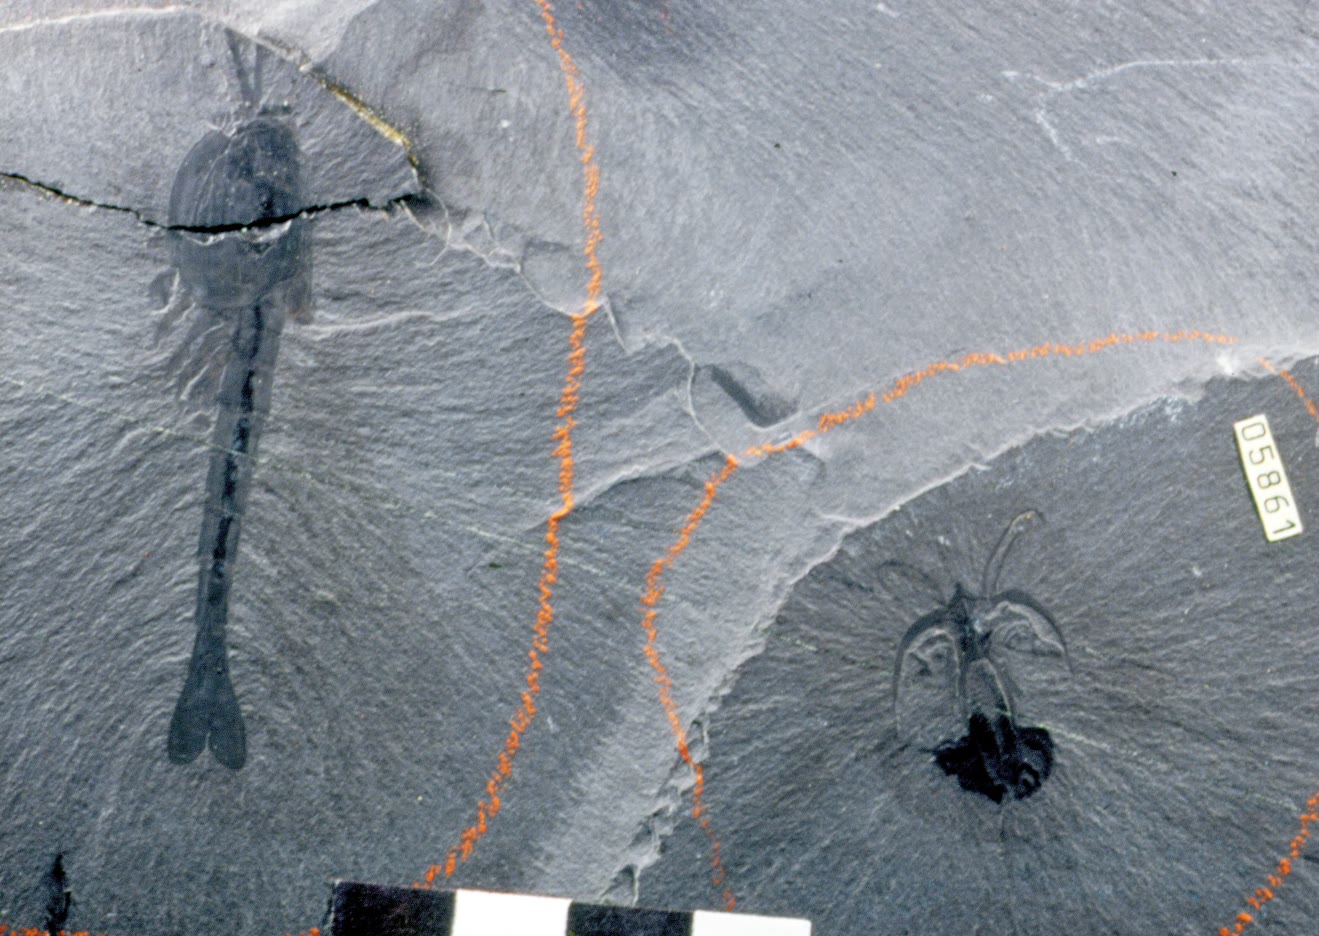
\includegraphics[width=0.72\linewidth]{images/book4/b2-20-burgess-waptia-marrella.jpg}
\par\smallskip{\small Two arthropods of the Burgess Shale, preserved as dark films of carbon:
\emph{Waptia} (left) and \emph{Marrella} (right). (James
St.~John, CC~BY~2.0, via Wikimedia Commons.)}
\end{omfigure}
% ledger: mussini25:burgess

\subsection*{Solnhofen}

The fine-grained limestones of Solnhofen and Eichstätt, in Bavaria, were laid down in lagoons
early in the Tithonian, the last age of the Jurassic, which began \qty{149.2}{Ma} ago. They are
the type locality of twelve specimens of \emph{Archaeopteryx}, of many pterosaurs and of fish
whose soft tissues and even colour patterns survive. Fossils there are rare, but their
preservation is outstanding. Several conditions have been proposed, perhaps acting together:
bottom waters about three times saltier than sea water or very alkaline, which slow bacterial
decay; mats of bacteria that sealed the carcasses; oxygen-free bottom water, which kept
scavengers away; and storms that stirred up the lime mud and buried the carcasses quickly. Each
of them lengthens the survival time $1/k$ or shortens the time to burial $h/s$.
% ledger: gerschermann21:solnhofen, rauhut18:archaeopteryx, ics4:jurassic-stages

\begin{omfigure}
\centering
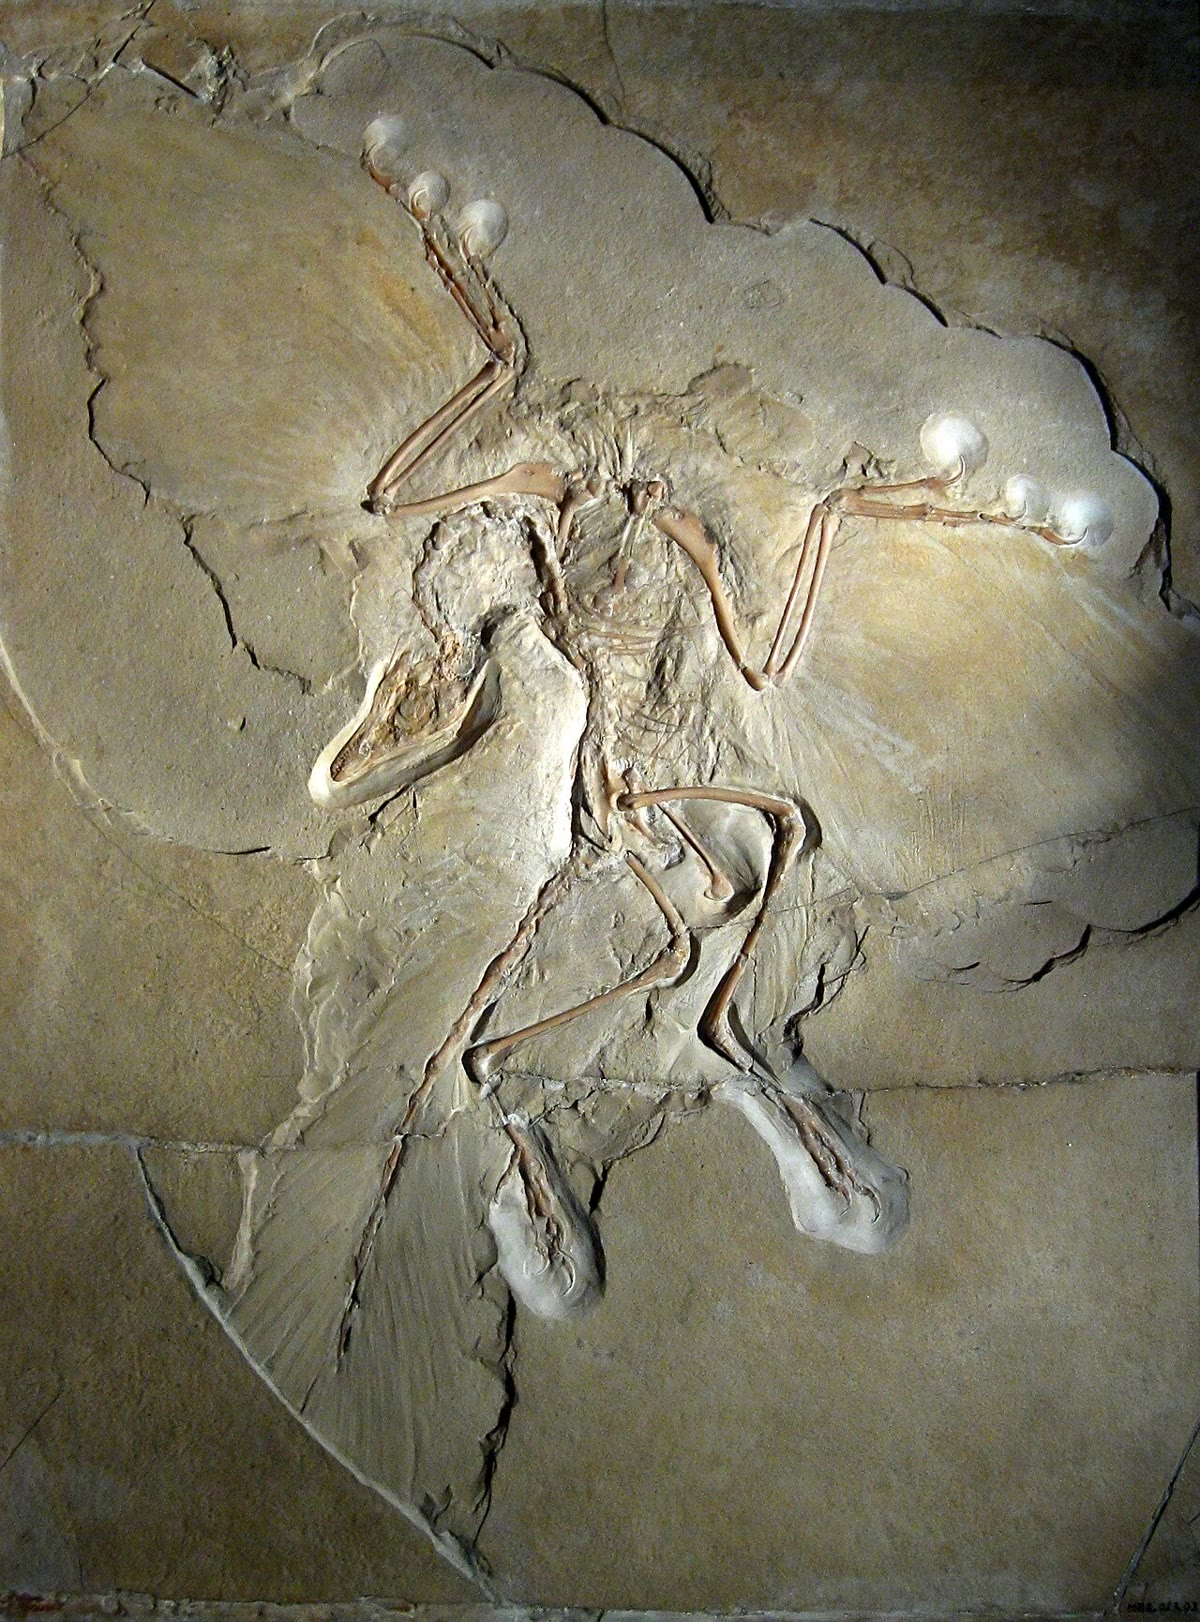
\includegraphics[width=0.5\linewidth]{images/book4/b2-20-archaeopteryx-berlin.jpg}
\par\smallskip{\small The Berlin specimen of \emph{Archaeopteryx}, from the Solnhofen
limestones: the bones and the imprints of the feathers of wings and tail. (H.~Raab, CC~BY-SA~3.0,
via Wikimedia Commons.)}
\end{omfigure}
% ledger: rauhut18:archaeopteryx, gerschermann21:solnhofen

\subsection*{Fossils as clocks}

The Year 1 volume built the biozone, a body of strata defined by its fossils, and the index
fossil that recognises it. How fine a clock do they make? A Jurassic ammonite zone can last
about a million years: the earliest Toarcian zone, dated with uranium--lead ages of ash beds in
Argentina, spans 183.73 to \qty{182.77}{Ma}. Zones are divided into horizons, and in the Late
Jurassic an ammonite horizon lasts on average \qty{165}{kyr}. All the skeletons of
\emph{Archaeopteryx} come from a single zone that holds five horizons, so the bird is known over
some 0.7 to 1 million years. The fossils, however, give only an order; the ages in years come
from ash beds dated by uranium and lead, and from sedimentary cycles. The same ash beds put the base of the Toarcian at $183.73$, with an uncertainty of
$+0.35$ and \qty{-0.50}{Myr}, where the international chart gives \qty{184.2}{Ma}.
% ledger: alsuwaidi22:toarcian, rauhut18:archaeopteryx, ics4:jurassic-stages

\section{Fossils as witnesses of environment}\label{sec:b2:palaeoenvironments:environment}

To read an environment in a fossil, a geologist assumes that the organism lived where its living
relatives live, and that the processes that act on sediment today acted in the same way then.

\begin{definition}[Actualism]\label{def:b2:palaeoenvironments:actualism}
\emph{Actualism}\index{actualism} is the method of interpreting past geological records by the
processes, and the relations between organisms and their environment, that can be observed today.
\end{definition}

In 1830 Charles Lyell gave the first volume of his \emph{Principles of Geology} the subtitle ``an
attempt to explain the former changes of the Earth's surface, by reference to causes now in
operation''. The method has limits. Many groups are extinct, and their way of life must be
inferred from their shape and from the sediment around them; and an environment of the past may
have no exact counterpart today.
% ledger: lyell1830:title

\begin{definition}[Palaeoenvironment]\label{def:b2:palaeoenvironments:palaeoenvironment}
A \emph{palaeoenvironment}\index{palaeoenvironment} is the set of physical, chemical and
biological conditions that prevailed where and when a rock formed: the setting, the depth and
energy of the water, its salinity, temperature and oxygen, the nature of the floor, and the life
on it.
\end{definition}

\subsection*{Where did the fossil live?}

The first question is whether the fossils lived where they lie.

\begin{definition}[Life and death assemblages; autochthonous and allochthonous fossils]\label{def:b2:palaeoenvironments:assemblages}
A \emph{life assemblage}\index{life assemblage} is a group of fossils of organisms that lived
together, preserved where and as they lived; a \emph{death assemblage}\index{death assemblage} is
a group of remains brought together after death, which may mix organisms of different places
and different times. A fossil is \emph{autochthonous}\index{autochthonous fossil} if it is
preserved where the organism lived, and \emph{allochthonous}\index{allochthonous fossil} if it was
transported from elsewhere before burial.
\end{definition}

The clues are those of transport. Shells still closed, a coral or a burrowing bivalve in its
growth position, delicate spines intact, all ages of a population present: the fossils are
probably \omterm{def:b2:palaeoenvironments:assemblages}{autochthonous}. Single valves sorted by size, worn and broken fragments, shells
concentrated at the base of a graded bed: they were carried. A \omterm{def:b2:palaeoenvironments:assemblages}{death assemblage} of shells, like
the one on the coastal floor above, still holds most of the community, but it gathers many years
of it into one layer: its fossils are averaged over time.
% ledger: tyler25:live-dead

\subsection*{Salinity and oxygen}

Some animals tolerate only the salinity of the open sea: they are called stenohaline. Echinoderms,
cephalopods, corals and, in the Palaeozoic, trilobites are typical stenohaline groups; their
presence speaks for normal sea water, and their absence from a rich fauna can speak against it.
The deposits of a Silurian estuary in Vietnam hold plant debris, fish bones, bivalves, gastropods
and ostracods, but none of these groups. Echinoderms are also missing from the Chengjiang biota,
a \omterm{def:b2:palaeoenvironments:lagerstatte}{Lagerstätte} about 518 million years old, although they occur in open-marine Lagerstätten of the
Cambrian: the Chengjiang animals lived off a delta, where fresh water made the salinity fluctuate.
% ledger: mcgairy21:stenohaline, saleh22:echinoderms, saleh22:age

Oxygen leaves its mark through the burrowers. Where the bottom water has oxygen, animals mix the
sediment and destroy its fine lamination; where it has none, the laminae survive, burrows are
absent and pyrite forms, as in the black shales of the \omterm{def:b2:phanerozoic-earth:oae}{oceanic anoxic events} of
\cref{ch:b2:phanerozoic-earth}. The same lack of burrowers protected the carcasses of the Burgess
Shale.
% ledger: mussini25:burgess

\subsection*{Ichnofacies}

\omterm{def:b2:palaeoenvironments:fossil-kinds}{Trace fossils} are the best witnesses of the floor, because they were not moved. Their makers
respond to the energy of the water, the firmness of the floor, the food and the oxygen, and the
same associations of traces recur through the Phanerozoic.

\begin{definition}[Ichnofacies]\label{def:b2:palaeoenvironments:ichnofacies}
An \emph{ichnofacies}\index{ichnofacies} is a recurrent association of \omterm{def:b2:palaeoenvironments:fossil-kinds}{trace fossils} that
reflects a set of environmental conditions; it is named after a characteristic trace.
\end{definition}

Along a marine profile, from the shore to the deep basin, four marine \omterm{def:b2:palaeoenvironments:ichnofacies}{ichnofacies} follow one
another (figure below). The \emph{Skolithos} \omterm{def:b2:palaeoenvironments:ichnofacies}{ichnofacies}, dominated by vertical, cylindrical or
U-shaped dwelling burrows of suspension feeders, with few horizontal traces, is typical of the
foreshore and the shoreface. The \emph{Cruziana} \omterm{def:b2:palaeoenvironments:ichnofacies}{ichnofacies}, dominated by the burrows of
deposit feeders, with the traces of grazers, carnivores and suspension feeders, is typical of the
offshore: the floor between the fair-weather wave base, the depth above which ordinary waves stir
the sediment, and the storm wave base, reached only by storm waves. The \emph{Zoophycos}
\omterm{def:b2:palaeoenvironments:ichnofacies}{ichnofacies}, named after a burrow that reworks the sediment in helicoidal sheets around a central
axis, is typical of the shelf below the storm wave base and of the slope. The \emph{Nereites}
\omterm{def:b2:palaeoenvironments:ichnofacies}{ichnofacies}, with its regular meandering, spiral and network burrows, read as the traps and
gardens of animals that found little food, is typical of the deep sea beyond the shelf break. In
brackish bays and estuaries a Cruziana \omterm{def:b2:palaeoenvironments:ichnofacies}{ichnofacies} of few species is the rule.
% ledger: buatois20:ichnofacies, miguez21:ichnofacies, zhang15:zoophycos, buatois25:graphoglyptids, paz23:nereites

\begin{omfigure}
\centering
\begin{tikzpicture}[font=\scriptsize, x=1cm, y=1cm]
% sea and floor (schematic, not to scale)
\fill[omSea!20] (0.6,0) -- (14,0) -- (14,-3.6) -- (11.2,-3.6) -- (9.6,-1.9) -- (6.2,-1.5)
  -- (3.2,-0.9) -- (1.2,-0.15) -- cycle;
\fill[omLithSand!45] (0,0.25) -- (0.6,0) -- (1.2,-0.15) -- (3.2,-0.9) -- (6.2,-1.5)
  -- (9.6,-1.9) -- (11.2,-3.6) -- (14,-3.6) -- (14,-4.3) -- (0,-4.3) -- cycle;
\draw[black!70, line width=0.6pt] (0,0.25) -- (0.6,0) -- (1.2,-0.15) -- (3.2,-0.9) -- (6.2,-1.5)
  -- (9.6,-1.9) -- (11.2,-3.6) -- (14,-3.6);
\draw[omSea!80!black, line width=0.6pt] (0.6,0) -- (14,0);
\node[anchor=south east, omSea!80!black] at (14,0) {sea level};
% wave bases
\draw[dashed, black!60] (2.133,-0.5) -- (14,-0.5) node[anchor=south east, black!70] {fair-weather wave base};
\draw[dashed, black!60] (4.7,-1.2) -- (14,-1.2) node[anchor=south east, black!70] {storm wave base};
% zone labels
\node[align=center] at (1.9,0.55) {foreshore,\\shoreface};
\node[align=center] at (4.6,0.55) {offshore};
\node[align=center] at (8.0,0.55) {shelf};
\node[align=center] at (10.5,0.55) {slope};
\node[align=center] at (12.7,0.55) {basin};
% Skolithos: vertical tubes
\foreach \x in {1.75,1.95,2.15,2.35} {\draw[black!80, line width=0.7pt] (\x,{-0.15-0.375*(\x-1.2)}) -- ++(0,-0.55);}
\node[align=center] at (2.1,-2.15) {\textbf{\emph{Skolithos}}\\vertical tubes};
% Cruziana: horizontal bilobed trails
\foreach \x in {4.0,4.8} {\draw[black!80, line width=0.6pt] (\x,-1.45) .. controls ++(0.2,0.08) .. ++(0.5,0);
  \draw[black!80, line width=0.6pt] (\x,-1.53) .. controls ++(0.2,-0.08) .. ++(0.5,0);}
\node[align=center] at (4.7,-2.35) {\textbf{\emph{Cruziana}}\\feeding burrows,\\grazing traces};
% Zoophycos: spreite arcs
\foreach \r in {0.12,0.22,0.32} {\draw[black!80, line width=0.5pt] (8.0,-2.25) ++(-\r,0) arc (180:360:\r cm and 0.5*\r cm);}
\draw[black!80, line width=0.6pt] (8.0,-2.25) -- (8.0,-1.8);
\node[align=center] at (8.0,-3.05) {\textbf{\emph{Zoophycos}}\\helicoidal\\sheets};
% Nereites: meander
\draw[black!80, line width=0.6pt, domain=0:2.2, samples=80, smooth] plot (12.0+\x*0.5,{-3.9+0.12*sin(\x*720)});
\node[align=center, anchor=north] at (12.5,-4.35) {\textbf{\emph{Nereites}}\\meanders, networks};
\end{tikzpicture}
\par\smallskip{\small The four marine \omterm{def:b2:palaeoenvironments:ichnofacies}{ichnofacies} of Seilacher's model along a profile from the
shore to the deep basin, with a sketch of a characteristic trace of each; depths are not to
scale. The traces respond to energy, food and oxygen more than to depth as such.}
\end{omfigure}
% ledger: buatois20:ichnofacies, miguez21:ichnofacies, zhang15:zoophycos, buatois25:graphoglyptids, paz23:nereites

Depth does not act directly. In a deep-sea channel, where turbidity currents are strong, vertical
burrows of the Skolithos \omterm{def:b2:palaeoenvironments:ichnofacies}{ichnofacies} appear far below any wave base; and near a delta, where fresh
water and mud pour in, the offshore traces are poorer than elsewhere. The makers also moved
through time: the burrow \emph{Zoophycos} lived on the shelf in the Palaeozoic, on the lower shelf
and the slope in the Mesozoic, and in the deep sea in the Cenozoic. An \omterm{def:b2:palaeoenvironments:ichnofacies}{ichnofacies} records the
conditions on the floor, from which the depth is only inferred, and the inference must use
the age of the rock.
% ledger: buatois20:ichnofacies, zhang15:zoophycos

\begin{inthefield}[Counting fossils bed by bed]
A palaeontologist who reconstructs an environment from a section logs each bed with its
lithology, thickness and sedimentary structures, and then its fossils: which groups, how many,
whether shells are whole or broken, closed or open, sorted or not, and in what position they lie.
\omterm{def:b2:palaeoenvironments:fossil-kinds}{Trace fossils} are recorded where they are seen, on the bedding surfaces and in the vertical faces,
with the depth to which the burrows reach. Because a shell can be moved but a burrow cannot, the
two lists are kept apart; the environment is read from the traces first, and the \omterm{def:b2:palaeoenvironments:fossil-kinds}{body fossils}
are then checked for signs of transport.
\end{inthefield}

\begin{omfigure}
\centering
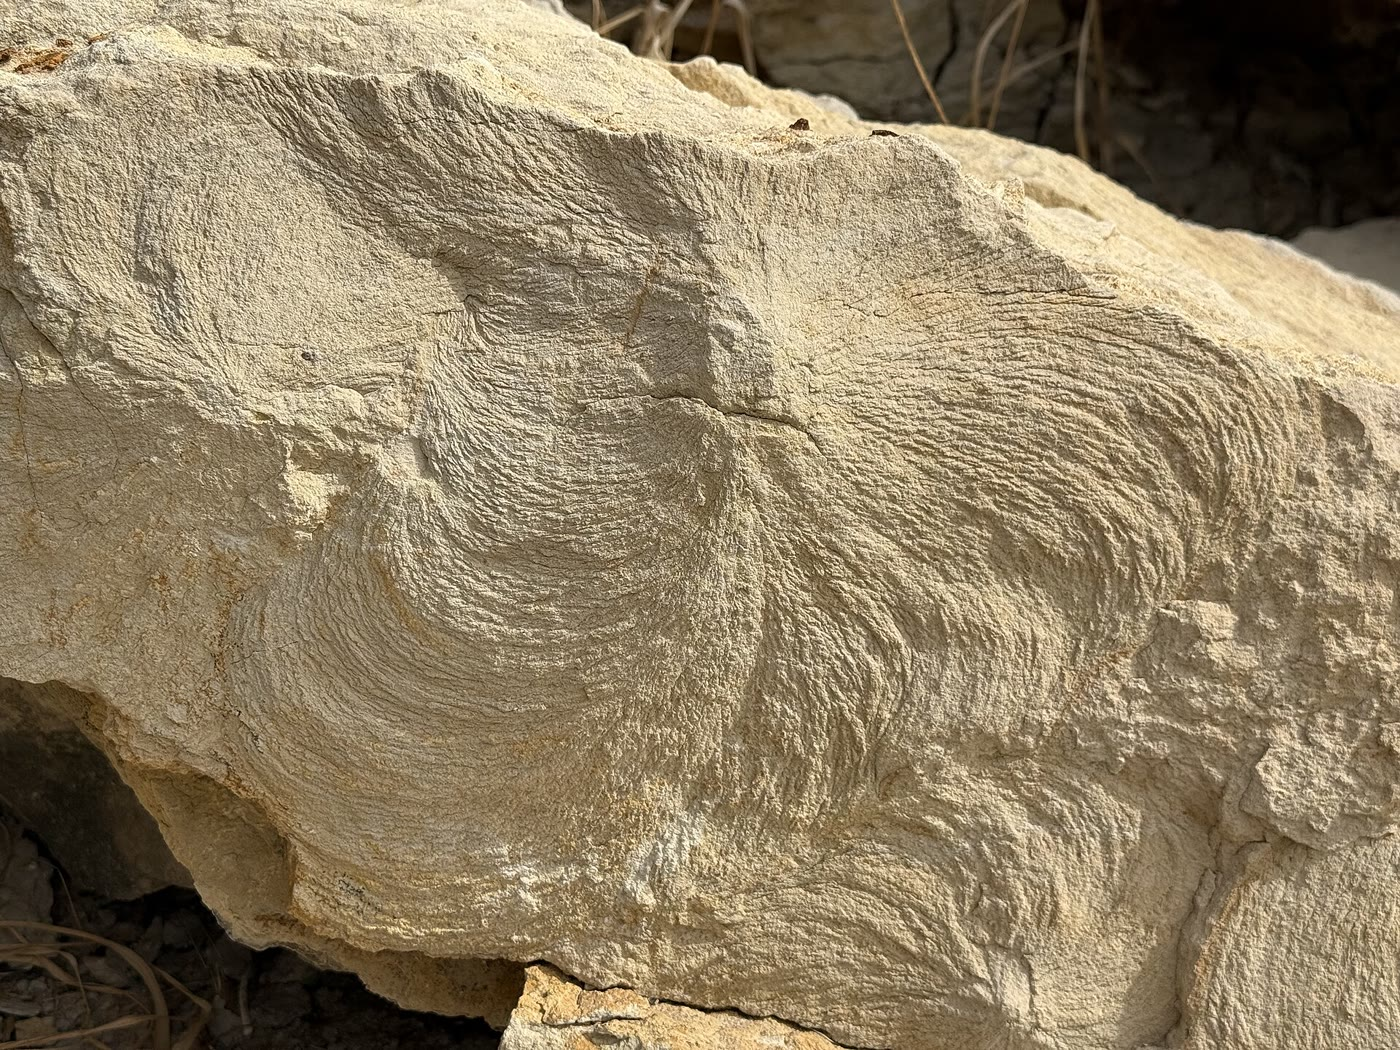
\includegraphics[width=0.5\linewidth]{images/book4/b2-20-zoophycos.jpg}
\par\smallskip{\small \emph{Zoophycos} in a block at Sagres, Portugal: the arcs are the lamellae
of a helicoidal sheet of reworked sediment. (Amada44, CC~BY~4.0, via Wikimedia Commons.)}
\end{omfigure}
% ledger: zhang15:zoophycos

\section{Reading a vanished sea}\label{sec:b2:palaeoenvironments:varden}

Environments lie side by side: a beach, an offshore floor, a deeper shelf. When the sea rises or
the floor sinks, each environment moves landward over its neighbour, and its deposits come to lie
on top of those of the neighbour. A vertical succession of facies, without a break, thus repeats
the order of the environments that lay next to each other; the Year 3 volume makes this rule,
Walther's law, its starting point. A log read from the bottom up is a film of the coast moving
across one place.

The cover of the Varden Hills, the series' invented region, makes a complete example. Its
thicknesses are those of the region's model; the fossils of the figure below are invented for it,
but each is chosen to be one that real rocks of that kind can hold. The limestone is given the
Toarcian, from 184.2 to \qty{174.7}{Ma}, and the shale the Aalenian to the Callovian, from
\qty{174.7}{Ma} to \qty{161.5}{Ma}.
% ledger: data:b4-palaeoenv, ics4:jurassic-stages

\begin{omfigure}
\centering
% figdata/bachelor-2/palaeoenv.py part log (thicknesses from figdata/shared/region.py)
\begin{tikzpicture}[x=1cm, y=0.0165cm, font=\scriptsize]
% scale
\draw[black!70] (-0.35,0) -- (-0.35,460);
\foreach \z in {0,100,...,400} {\draw[black!70] (-0.45,\z) -- (-0.35,\z) node[left=3pt] {\z};}
\node[rotate=90, anchor=south] at (-1.15,230) {height above the base of the cover (m)};
% units
\fill[lith sandstone] (0,0) rectangle (2.2,120);
\fill[lith limestone] (0,120) rectangle (2.0,180);
\fill[lith limestone] (0,180) rectangle (1.6,300);
\fill[lith shale] (0,300) rectangle (1.1,400);
\fill[om lith={icsCretaceous!35}{om limestone}] (0,400) -- (1.4,400) -- (1.4,452)
  .. controls (1.0,466) and (0.6,446) .. (0.3,458) -- (0,455) -- cycle;
\draw[black!70] (0,0) rectangle (2.2,120);
\draw[black!70] (0,120) rectangle (2.0,180);
\draw[black!70] (0,180) rectangle (1.6,300);
\draw[black!70] (0,300) rectangle (1.1,400);
\draw[black!70] (0,400) -- (1.4,400) -- (1.4,452) .. controls (1.0,466) and (0.6,446) ..
  (0.3,458) -- (0,455) -- cycle;
\node[anchor=west, font=\tiny] at (1.45,460) {eroded top};
% unit names
\node[anchor=west, align=left] at (2.6,60) {\textbf{sandstone}, \qty{120}{m}\\Triassic};
\node[anchor=west, align=left] at (2.6,150) {\textbf{oolitic limestone}, \qty{60}{m}\\Toarcian};
\node[anchor=west, align=left] at (2.6,240) {\textbf{fine limestone}, \qty{120}{m}\\Toarcian};
\node[anchor=west, align=left] at (2.6,350) {\textbf{shale}, \qty{100}{m}\\Aalenian--Callovian};
\node[anchor=west, align=left] at (2.6,424) {\textbf{chalk}\\Cretaceous};
% content
\node[anchor=west, align=left, text width=6.9cm] at (6.3,60) {cross-bedded channel fills on scoured
  bases; root traces; plant fragments; no marine fossils};
\node[anchor=west, align=left, text width=6.9cm] at (6.3,150) {cross-bedded ooids; vertical tubes
  and U-shaped burrows; worn shell fragments};
\node[anchor=west, align=left, text width=6.9cm] at (6.3,240) {crinoid ossicles, brachiopods,
  belemnites, ammonites; crawling trails and feeding burrows; beds of broken shells with sharp
  bases};
\node[anchor=west, align=left, text width=6.9cm] at (6.3,350) {dark grey, laminated in places;
  pyrite; ammonites and thin-shelled bivalves; helicoidal spreite burrows in the paler beds};
\node[anchor=west, align=left, text width=6.9cm] at (6.3,424) {coccoliths; echinoids, sponges;
  flint nodules; burrowed throughout};
\foreach \z in {120,180,300,400} {\draw[black!25] (2.25,\z) -- (13.2,\z);}
\node[font=\scriptsize\bfseries, anchor=south west] at (2.6,462) {unit and age};
\node[font=\scriptsize\bfseries, anchor=south west] at (6.3,462) {what the beds hold};
\end{tikzpicture}
\par\smallskip{\small The cover of the Varden Hills as a log, with the content of its units. The
thicknesses are those of the region's model, except the chalk, whose eroded top is cut short here
(\qty{766}{m} thick in the syncline of \cref{ex:b2:palaeoenvironments:shale}); the width of the column grows with the grain size;
the fossils and their ages are invented for the region.}
\end{omfigure}
% ledger: data:b4-palaeoenv, ics4:jurassic-stages

\begin{example}[The base of the Varden cover]\label{ex:b2:palaeoenvironments:base}
The sandstone holds channel fills on scoured bases, roots and plant fragments, and no marine
fossil: it was laid down by rivers on land. The oolitic limestone above has cross-bedded ooids,
which grow as they roll in agitated water, vertical tubes and U-shaped burrows of the Skolithos
\omterm{def:b2:palaeoenvironments:ichnofacies}{ichnofacies}, and worn shell fragments, all \omterm{def:b2:palaeoenvironments:assemblages}{allochthonous}: a shoal of the shoreface,
swept by waves. Between the two the sea arrived: the contact records a \omterm{def:b2:phanerozoic-earth:transgression}{marine transgression}. In
the order of Walther's law, the river plain was followed by the shore, then the shoal.
\end{example}
% ledger: buatois20:ichnofacies

\subsection*{How fast did the sea floor fill?}

A biozone gives a duration, a log gives a thickness, and their ratio is a rate. But the
thickness has shrunk since the sediment was laid down: the water of the pores has been squeezed
out, and the grains alone are conserved.

\begin{proposition}[Accumulation rate of a compacted layer]\label{prop:b2:palaeoenvironments:rate}
A layer of present thickness $h$ and mean porosity $\varphi$, laid down over the time $\Delta t$
with the porosity $\varphi_0$, accumulated at the rate
\[
  r = \frac{h\,(1 - \varphi)}{(1 - \varphi_0)\,\Delta t}
\]
of fresh sediment, and at the rate $h(1-\varphi)/\Delta t$ of grains, which does not depend on
$\varphi_0$.
\end{proposition}

\begin{proof}
Per unit area, the layer holds the volume of grains $h(1 - \varphi)$, the solid thickness of the
Year 1 volume. Compaction drives out water but neither adds nor removes grains, so the fresh
sediment, of porosity $\varphi_0$, had the thickness $h_0$ with $h_0(1 - \varphi_0) = h(1 -
\varphi)$. Dividing $h_0$ and the solid thickness by $\Delta t$ gives the two rates.
\end{proof}

When the porosity was not measured, Athy's law gives it from the depth. The figure below shows
the law for four lithologies, and the factor $(1 - \varphi(z))/(1 - \varphi_0)$ by which a thin
layer now at the depth $z$ must be stretched to give its thickness at the surface. Chalk and shale
start with much water and lose it fast: a thin layer of shale at \qty{1000}{m} was 1.68 times
thicker when it was laid down, a layer of chalk 2.19 times.
% ledger: pybacktrack:compaction, pybacktrack4:limestone, data:b4-palaeoenv

\begin{omfigure}
\centering
% figdata/bachelor-2/palaeoenv.py parts poro and ratio
\begin{tikzpicture}
\begin{groupplot}[group style={group size=2 by 1, horizontal sep=1.6cm},
  width=0.46\linewidth, height=6.2cm, y dir=reverse, ymin=0, ymax=3000,
  tick label style={font=\scriptsize}, label style={font=\small}, xtick pos=bottom,
  ytick pos=left, scaled y ticks=false, yticklabel style={/pgf/number format/1000 sep={\,}}]
\nextgroupplot[xmin=0, xmax=0.75, xlabel={porosity $\varphi$}, ylabel={depth $z$ (\unit{m})},
  legend style={at={(0.5,1.04)}, anchor=south, draw=none, font=\scriptsize, legend columns=2}]
\addplot[omThm, line width=1pt] table[x=shale, y=z_m] {figdata/out/bachelor-2-palaeoenv-poro.dat};
\addlegendentry{shale}
\addplot[omSea!80!black, line width=1pt, dashed] table[x=sandstone, y=z_m] {figdata/out/bachelor-2-palaeoenv-poro.dat};
\addlegendentry{sandstone}
\addplot[black, line width=1pt, dotted] table[x=chalk, y=z_m] {figdata/out/bachelor-2-palaeoenv-poro.dat};
\addlegendentry{chalk}
\addplot[green!45!black, line width=1pt, dash dot] table[x=limestone, y=z_m] {figdata/out/bachelor-2-palaeoenv-poro.dat};
\addlegendentry{limestone}
\nextgroupplot[xmin=1, xmax=3.2, xlabel={restoration factor $(1-\varphi)/(1-\varphi_0)$}]
\addplot[omThm, line width=1pt] table[x=shale, y=z_m] {figdata/out/bachelor-2-palaeoenv-ratio.dat};
\addplot[omSea!80!black, line width=1pt, dashed] table[x=sandstone, y=z_m] {figdata/out/bachelor-2-palaeoenv-ratio.dat};
\addplot[black, line width=1pt, dotted] table[x=chalk, y=z_m] {figdata/out/bachelor-2-palaeoenv-ratio.dat};
\addplot[green!45!black, line width=1pt, dash dot] table[x=limestone, y=z_m] {figdata/out/bachelor-2-palaeoenv-ratio.dat};
\end{groupplot}
\end{tikzpicture}
\par\smallskip{\small Left: porosity against depth by Athy's law, with the constants of Sclater
and Christie (1980) for shale, sandstone and chalk and of Turer and Maynard (2003) for limestone,
as tabulated in pyBacktrack. Right: the factor by which a thin layer at the depth $z$ is
restored to its thickness at the surface.}
\end{omfigure}
% ledger: pybacktrack:compaction, pybacktrack4:limestone, data:b4-palaeoenv

\begin{example}[The Varden shale]\label{ex:b2:palaeoenvironments:shale}
In the syncline of the Varden Hills the chalk is \qty{766}{m} thick, so the shale lies between
766 and \qty{866}{m}. With the constants of shale, $\varphi_0 = 0.63$ and $\lambda =
\qty{1960}{m}$, the solid thickness of the Year 1 volume is $100 - 0.63 \times 1960 \times
(e^{-766/1960} - e^{-866/1960}) = \qty{58.4}{m}$, a mean porosity of 0.416. Brought back to the
surface with the same grains, the layer is \qty{148.6}{m} thick. Over the \qty{13.2}{Myr} from
the base of the Aalenian to the top of the Callovian, the shale accumulated at $100/13.2 =
\qty{7.6}{m}$ per million years as it now stands, at $148.6/13.2 = \qty{11.3}{m}$ per million
years of fresh mud, and at \qty{4.4}{m} per million years of grains. The present thickness
understates the rate by a third.
\end{example}
% ledger: data:b4-palaeoenv, pybacktrack:compaction, ics4:jurassic-stages

The shale may once have lain deeper still, under chalk since eroded; the correction is then a
minimum. The weekend problem applies the proposition to the limestone, where the porosity was
measured.

\section*{Exercises}\label{sec:b2:palaeoenvironments:exercises}

Data for the exercises, unless stated otherwise: Athy's law $\varphi = \varphi_0 e^{-z/\lambda}$
with $\varphi_0 = 0.63$, $\lambda = \qty{1960}{m}$ (shale), $0.49$, \qty{3704}{m} (sandstone),
$0.70$, \qty{1408}{m} (chalk), $0.51$, \qty{4545}{m} (limestone); calcite \qty{2710}{kg.m^{-3}},
pore water \qty{1000}{kg.m^{-3}}; the ages of the international chart: Toarcian 184.2 to
\qty{174.7}{Ma}.
% ledger: pybacktrack:compaction, pybacktrack4:limestone, ics4:jurassic-stages

\begin{exercise}[$\star$]\label{exo:b2:palaeoenvironments:1}
At 51 sites of a coastal floor, 135 species of invertebrates were found alive, 150 among the dead
shells and skeletons on the floor, and 112 that also have a fossil record. (a) Express the third
number as a fraction of each of the first two. (b) How can the dead outnumber the living? (c)
Which feeding groups would you expect to be under-represented among the dead, and why?
\end{exercise}
% ledger: tyler25:live-dead, tyler25:soft-bodied

\begin{exercise}[$\star$]\label{exo:b2:palaeoenvironments:2}
A Late Jurassic ammonite horizon lasts on average \qty{165}{kyr}. (a) How long do five horizons
last? Compare with the 0.7 to 1 million years given for \emph{Archaeopteryx}. (b) The earliest
Toarcian zone spans 183.73 to \qty{182.77}{Ma}: how many horizons of average length would it hold?
(c) Why do horizons, not zones, matter for following the evolution of a lineage?
\end{exercise}
% ledger: rauhut18:archaeopteryx, alsuwaidi22:toarcian

\begin{exercise}[$\star$]\label{exo:b2:palaeoenvironments:3}
Name the \omterm{def:b2:palaeoenvironments:ichnofacies}{ichnofacies} and the setting of each suite. (a) Meandering grazing trails and regular
burrow networks on the soles of thin turbidites. (b) Closely spaced vertical tubes in clean,
cross-bedded sand. (c) Abundant horizontal burrows of deposit feeders and grazing traces in silty
beds between storm sands. (d) Helicoidal spreite burrows in a fine, dark mud with no wave
ripples, in Mesozoic rocks.
\end{exercise}
% ledger: buatois20:ichnofacies, paz23:nereites

\begin{exercise}[$\star$]\label{exo:b2:palaeoenvironments:4}
Bed A holds crinoids, brachiopods, corals and trilobites; bed B, of the same age, holds plant
debris, fish bones, a few bivalves and gastropods, and many individuals of only two species of
ostracods. (a) What does each say about the salinity of its water? (b) Bed B lacks the groups of
bed A: why is that absence an argument, while the absence of one fossil from one bed is not?
(c) Which other observations would test the interpretation of bed B?
\end{exercise}
% ledger: mcgairy21:stenohaline, saleh22:echinoderms

\begin{exercise}[$\star\star$]\label{exo:b2:palaeoenvironments:5}
Use \cref{prop:b2:palaeoenvironments:burial} with the shell of
\cref{ex:b2:palaeoenvironments:shell}, $k = \qty{0.05}{yr^{-1}}$ and $h = \qty{0.1}{m}$. (a)
Find the sedimentation rate at which half the shells reach safety. (b) By what factor does $P$
change when the rate is halved from that value? (c) A shell twice as thick survives twice as long
on the floor. At \qty{1}{mm.yr^{-1}}, how much more likely is it to be preserved? (d) What does
this imply for the proportions of thin and thick shells in a fossil assemblage?
\end{exercise}
% ledger: tyler25:soft-bodied

\begin{exercise}[$\star\star$]\label{exo:b2:palaeoenvironments:6}
Ash beds date the base of the Toarcian at Chacay Melehue to $183.73$, $+0.35$, \qty{-0.50}{Myr};
the international chart gives \qty{184.2}{Ma}. (a) Is the chart's value within the uncertainty?
By how much does it miss the upper bound? (b) The earliest Toarcian zone ends at
\qty{182.77}{Ma}: find its duration. (c) Suppose this zone is \qty{6}{m} thick in a section:
what is the rate of accumulation? (d) Why can a biozone be the same everywhere in time while its
thickness differs from place to place?
\end{exercise}
% ledger: alsuwaidi22:toarcian, ics4:jurassic-stages

\begin{exercise}[$\star\star$]\label{exo:b2:palaeoenvironments:7}
In the Varden syncline the sandstone lies between 1046 and \qty{1166}{m} below the ground. (a)
Find its porosity by Athy's law at the top and at the base, and its mean porosity, rounded to
three decimals, from the average of the two. (b) Find its solid thickness. (c) Restore it to the
surface with the thin-layer factor at the mean porosity. (d) The exact restoration gives
\qty{147.0}{m}. Why is the thin-layer estimate a little too large?
\end{exercise}
% ledger: data:b4-palaeoenv, pybacktrack:compaction

\begin{exercise}[$\star\star$]\label{exo:b2:palaeoenvironments:8}
A density log reads \qty{2573}{kg.m^{-3}} in the Varden limestone, made of calcite grains with
water in the pores. (a) Show that the porosity is $\varphi = (\rho_{\text{grain}} -
\rho)/(\rho_{\text{grain}} - \rho_{\text{water}})$ and compute it. (b) At the mid-depth of the
limestone in the syncline, \qty{956}{m}, what does Athy's law predict with the limestone constants?
(c) Which process of diagenesis can explain the difference?
\end{exercise}
% ledger: pybacktrack4:limestone, data:b4-palaeoenv

\begin{exercise}[$\star\star$]\label{exo:b2:palaeoenvironments:9}
A cliff of Jurassic rocks shows from the base up: thin turbidites with regular meanders and burrow
networks; dark mud with helicoidal spreite burrows; silty beds with deposit-feeder burrows between
storm sands; clean cross-bedded sand with
vertical tubes; then a coal with roots. (a) Interpret each part. (b) Did the water deepen or
shallow? (c) Name two causes that could produce this succession, and say what would decide
between them. (d) Why is a sharp jump from the first part to the fourth, without the others, a
warning?
\end{exercise}
% ledger: buatois20:ichnofacies, paz23:nereites

\begin{exercise}[$\star\star\star$]\label{exo:b2:palaeoenvironments:10}
A soft-bodied animal survives on the floor for a year on average ($k = \qty{1}{yr^{-1}}$), a
shell for a century; both are safe under $h = \qty{0.1}{m}$. (a) Compare their chances of
preservation at 1, 10 and \qty{100}{mm.yr^{-1}}. (b) Find the rate at which one soft body in a
hundred is preserved. (c) Is such a rate plausible for months on end? What kind of deposit buries
the floor faster? (d) Which assumption of \cref{prop:b2:palaeoenvironments:burial} fails for such
a deposit, and how does the formula behave when it fails?
\end{exercise}

\begin{exercise}[$\star\star\star$]\label{exo:b2:palaeoenvironments:11}
(a) Show that the thin-layer factor $(1 - \varphi(z))/(1 - \varphi_0)$ follows from
\cref{prop:b2:palaeoenvironments:rate}. (b) Apply it at the mid-depth of the Varden shale,
\qty{816}{m}, to restore the \qty{100}{m} of shale. (c) Compare with the exact \qty{148.6}{m} of
\cref{ex:b2:palaeoenvironments:shale}, and explain the sign of the difference. (d) Show that the
rate of grains, unlike the rate of fresh sediment, can be compared between a shale and a limestone
without knowing how porous each was when laid down.
\end{exercise}
% ledger: data:b4-palaeoenv, pybacktrack:compaction

\begin{exercise}[$\star\star\star$]\label{exo:b2:palaeoenvironments:12}
Suppose the Toarcian ammonite horizons last \qty{165}{kyr} on average, like Late Jurassic ones.
(a) How many horizons would the \qty{180}{m} of the Varden limestone hold? (b) What thickness of
limestone does one horizon represent today, and what thickness of fresh sediment, given that the
layer was \qty{338}{m} thick when laid down? (c) To be sure of finding every horizon, a
geologist samples at no more than half that present thickness: what spacing is that, and how many
samples? (d) Why might some horizons be missing even so?
\end{exercise}
% ledger: rauhut18:archaeopteryx, ics4:jurassic-stages, data:b4-palaeoenv

\begin{problem}[{Weekend problem --- The Jurassic sea of the Varden Hills}]\label{pb:b2:palaeoenvironments:1}
This problem reads the environment and the history of the Varden cover, with the log of
\cref{sec:b2:palaeoenvironments:varden} and the data of the exercises. The cover dips at
\ang{12} on the limbs of the folds; in the syncline it is drilled through by a well.

\medskip\noindent\textbf{Part I --- The rocks and their thickness.}
\begin{enumerate}
  \item On level ground on a limb, the limestone crops out over a width of \qty{866}{m}, measured
        across the strike. Find its true thickness.
  \item The shale crops out over \qty{481}{m}. Find its thickness.
  \item Which unit is the oldest, and on what principle?
  \item In the well, the shale starts at \qty{766}{m}, the limestone at \qty{866}{m} and the
        sandstone at \qty{1046}{m} below the ground. Check the thicknesses.
  \item The chalk is cut by the ground surface. What can be said of its thickness when the
        Cretaceous sea withdrew?
  \item Find the porosity of the chalk at the surface and at the base of the chalk in the well.
\end{enumerate}

\medskip\noindent\textbf{Part II --- Environments.}
\begin{enumerate}[resume]
  \item What do the crinoids, brachiopods, belemnites and ammonites of the fine limestone say
        about its water?
  \item Which \omterm{def:b2:palaeoenvironments:ichnofacies}{ichnofacies} do its traces form, and in which part of the profile?
  \item What do its beds of broken shells with sharp bases record?
  \item The shale is dark, laminated in places, with pyrite and few burrows. What does that say
        about the bottom water?
  \item Its paler beds hold helicoidal spreite burrows. Which \omterm{def:b2:palaeoenvironments:ichnofacies}{ichnofacies}, and which setting?
  \item Are the ammonites of the shale part of a \omterm{def:b2:palaeoenvironments:assemblages}{life assemblage} of the floor? Explain.
\end{enumerate}

\medskip\noindent\textbf{Part III --- Time and rates.} The lowest limestone beds hold the
ammonites of the first Toarcian zone, the highest those of the last, and the shale begins with
the first Aalenian zone.
\begin{enumerate}[resume]
  \item How long did the limestone take to accumulate?
  \item At what rate, as the limestone now stands?
  \item The density log of the well reads \qty{2573}{kg.m^{-3}} in the limestone. Find its
        porosity.
  \item Lime mud is laid down with a porosity of 0.51. Find the thickness of the fresh sediment.
  \item Find the rate of fresh sediment.
  \item Find the rate of grains.
  \item Compare with the shale of \cref{ex:b2:palaeoenvironments:shale}. What does the change of
        rate suggest about the supply of carbonate?
\end{enumerate}

\medskip\noindent\textbf{Part IV --- The sea over Varden.}
\begin{enumerate}[resume]
  \item Read the column from the sandstone to the chalk. Did the sea advance or retreat?
  \item On the long-term curve of Haq and others, global sea level stood about 41, 57 and
        \qty{86}{m} above today's at 184, 174 and \qty{162}{Ma}. By how much did it rise over the
        limestone, over the shale, and in all?
  \item Suppose the floor went from \qty{5}{m} of water on the shoal to \qty{60}{m} at the top of
        the shale. Find the accommodation created from the base of the limestone to the top of the
        shale, counting the fresh thicknesses of both units, and its mean rate.
  \item What share of it can the global rise explain? What made the rest?
  \item To sum up: at what rate did the lime mud of the Varden limestone accumulate when it was
        laid down?
\end{enumerate}
\end{problem}
% ledger: data:b4-palaeoenv, ics4:jurassic-stages, pybacktrack4:limestone, pybacktrack:compaction, data:b4-sealevel, haq87:charts, buatois20:ichnofacies, mcgairy21:stenohaline
